\section{Introduction} \label{section:Introduction}

Light field (LF) images, unlike regular images captured by monocular cameras, provide richer information by capturing light rays from multiple angular directions in a single shot. This unique characteristic has paved the way for substantial progress in various computer vision applications where conventional cameras have shown limited efficacy, \textit{e.g.,} material recognition \cite{wangLFRecognition_ECCV2016, luLFRecognition_2019}, depth estimation \cite{yucer2016efficient, heberUshapeICCV2017, wangOcclusionawareDepthEstimation2015, chaoSubFocal_TCI2023, ding_TCI2023}, salient object detection under complex scenarios \cite{shengLFSaliency_ICASSP2016, zhangLFNet_TIP2020, chen_TMM2023}, microsopy \cite{verinaz_TCI2022, verinaz_TCI2023, levoy2006light}, and anti-spoof face recognition \cite{raghavendraLFFace_TIP2015, jiLFHOG_ICIP2016}. By simultaneously capturing multiple sub-aperture images (SAIs, or views), LF technology enables a rich and interactive viewing experience. Users can freely explore and interact with the virtual environments, changing perspectives and moving within them. Therefore, LF technology has become a cornerstone of VR applications, enhancing user engagement and immersion.


\newcommand{\imageWithGrid}[3]{%
  \begin{tikzpicture}
    \node[anchor=south west,inner sep=0] (image) at (0,0) {\includegraphics[width=#2, height=#3]{#1}};
    \begin{scope}[x={(image.south east)},y={(image.north west)}]
        \foreach \i in {1,...,4} {
            \draw[lightgray,thin] (\i/5,0) -- (\i/5,1); % Vertical lines
            \draw[lightgray,thin] (0,\i/5) -- (1,\i/5); % Horizontal lines
        }
        \draw[black] (0,0) rectangle (1,1);
    \end{scope}
  \end{tikzpicture}%
}


\begin{figure}[t!]
\centering

\tabcolsep=0.04cm
\renewcommand{\arraystretch}{0.8}
\begin{tabular}{ccccc}
    \raisebox{0.5\height}{
        \resizebox{0.05\textwidth}{!}{
        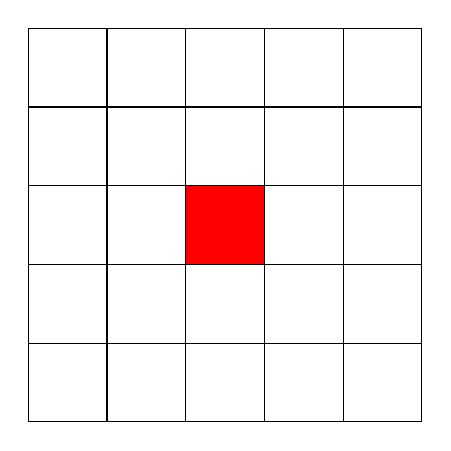
\begin{tikzpicture}
            \foreach \x in {0,1,2,3,4} {
                \foreach \y in {0,1,2,3,4} {
                    \draw[black, thin] (\x,\y) rectangle (\x+1,\y+1);
                }
            }
            \draw[black] (0,0) rectangle (5,5);
            \fill[red] (2,2) rectangle (3,3);
        \end{tikzpicture}}
    } &
    \includegraphics[width=0.09\textwidth]{img/qual/Perforated_Metal_3/LR.annotated.png} &
    \includegraphics[width=0.09\textwidth]{img/qual/Perforated_Metal_3/EPIT/SR.png} &
    \includegraphics[width=0.09\textwidth]{img/qual/Perforated_Metal_3/SAT/SR.png} &
    \includegraphics[width=0.09\textwidth]{img/qual/Perforated_Metal_3/HR.png} \\
    \footnotesize{\makecell{SAI\\Location}} & \footnotesize LR & \footnotesize EPIT & \footnotesize M2MT-Net & \footnotesize HR
\end{tabular} \\

(a) SAI location and patch images. \\
\hspace{0pt}

\tabcolsep=0.1cm
\begin{tabular}{cc}
    \imageWithGrid{img/qual/Perforated_Metal_3/EPIT/LAM.png}{0.18\textwidth}{0.18\textwidth} &
    \imageWithGrid{img/qual/Perforated_Metal_3/SAT/LAM.png}{0.18\textwidth}{0.18\textwidth} \\
    % \includegraphics[width=0.22\textwidth,cfbox=black 0.5pt 0pt]{img/qual/Perforated_Metal_3/EPIT/LAM.png} &
    % \includegraphics[width=0.22\textwidth,cfbox=black 0.5pt 0pt]{img/qual/Perforated_Metal_3/SAT/LAM.png} \\
    EPIT (DI: 5.9518) & M2MT (DI: 27.2578) \\
\end{tabular} \\
\vspace{8pt}
(b) Local attribution maps of SAIs: Diffusion Index (DI) quantifies the extent of influential pixels.\\
% From the original paper: The Diffusion Index (DI) reflects the range of involved pixels. A higher DI represents a wider range of attention.
%DI represents Diffusion Index.\\
\hspace{0pt}
\caption{Super-resolved results and local attribute maps (LAM) of the proposed M2MT-Net against the current state-of-the-art methods on the \textit{Perforated\_metal\_3} sample.}
% \caption{Illustration of super-resolved images and LAM comparing EPIT and M2MT on a patch of the \textit{Perforated metal 3} sample.}

\label{fig:First}
\end{figure}


Capturing LF images necessitated self-built dense camera arrays \cite{wilburn2004high, wilburn2005high}, which were prohibitively expensive and not ready for mainstream use. However, advancements of sophisticated LF cameras like Raytrix \cite{Raytrix}, Lytro Illum \cite{Lytro}, and Google's Light Field VR Camera \cite{GoogleLF} have gradually democratized LF imaging, making it accessible for both commercial and industrial applications. Despite this progress, LF cameras have long faced the challenges in striking a balance angular and spatial resolutions due to inherent limitations in sensor capabilities, often leading to lower spatial resolutions compared to traditional cameras.

Researchers have developed a number of possible solutions and they generally fall into two categories: light field image super-resolution (LFSR) \cite{yeungSAS_LFSR2019,wangDistgSSR_TIP2022} and light field angular super-resolution (also known as light field view synthesis) \cite{liu_TMM2022, yeungSAS_ECCV2018}. LFSR aims to upsample the spatial resolution of each SAI, effectively reconstructing the details within the views, which is the focus of this paper. On the other hand, light field angular super-resolution focuses on synthesizing additional SAIs to enhance the angular resolution of the light field. This paper primarily concentrates on LFSR.

\begin{figure*}[t!]
    \definecolor{myred}{HTML}{FF0080}
    \definecolor{myblue}{HTML}{007FFF}
    \centering

    \tabcolsep=0.10cm
    \renewcommand{\arraystretch}{0.1}
    \setlength{\medmuskip}{-1mu}
    \begin{tabular}{cc}
        \raisebox{0.025\height}{
        \includegraphics[width=0.250\linewidth]{img/cubes/LF.pdf}
        }
        &
        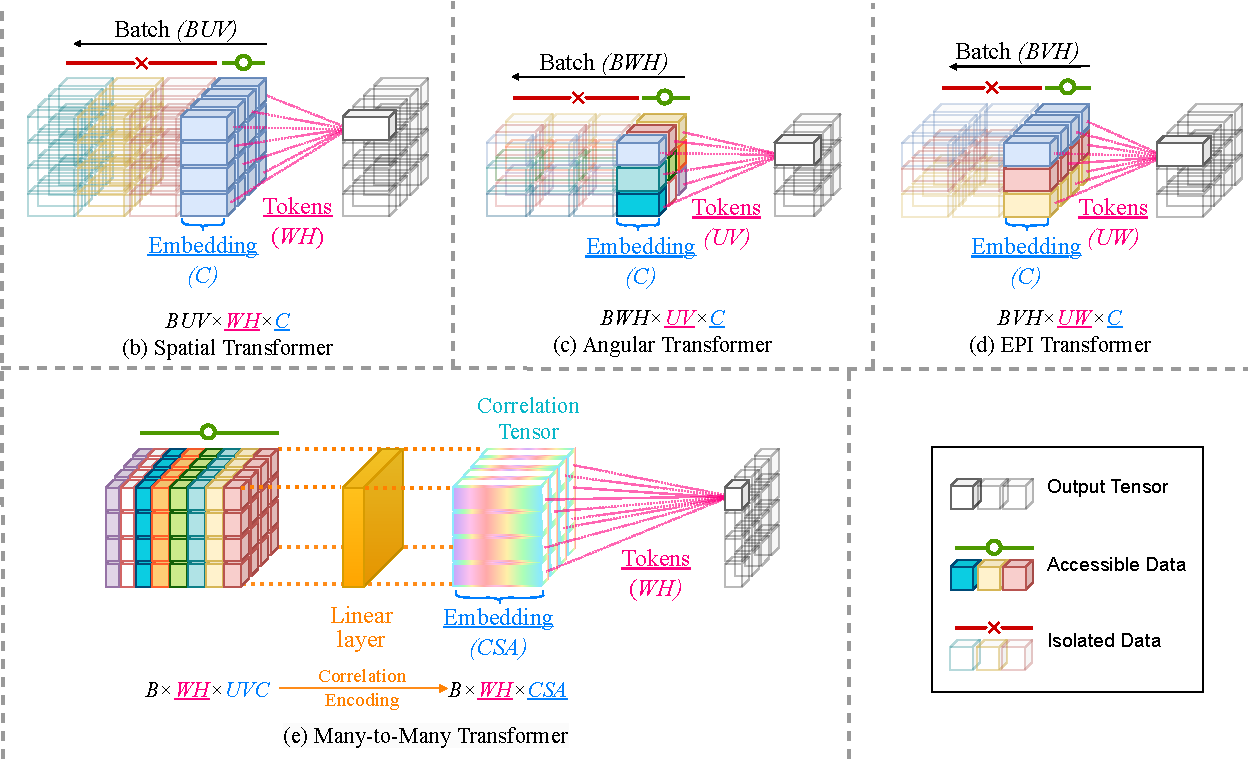
\includegraphics[width=0.660\linewidth]{img/cubes/main.pdf}
        % \begin{tabular}{ccc}
        %     \includegraphics[height=0.155\linewidth]{img/cubes/Spatial.pdf} &
        %     \includegraphics[height=0.155\linewidth]{img/cubes/Angular.pdf} &
        %     \includegraphics[height=0.155\linewidth]{img/cubes/EPI.pdf} \\
        %     \footnotesize $BU\!V \times \textcolor{myred}{\underline{W\!H}} \times \textcolor{myblue}{\underline{C}}$ &
        %     \footnotesize $BW\!H \times \textcolor{myred}{\underline{U\!V}} \times \textcolor{myblue}{\underline{C}}$ &
        %     \footnotesize $BV\!H \times \textcolor{myred}{\underline{U\!W}} \times \textcolor{myblue}{\underline{C}}$ \\
        %     \footnotesize (b) Spatial Transformer. &
        %     \footnotesize (c) Angular Transformer. &
        %     \footnotesize (d) EPI Transformer. \\
        %     \vspace{0pt} & \\
        %     \multicolumn{3}{c}{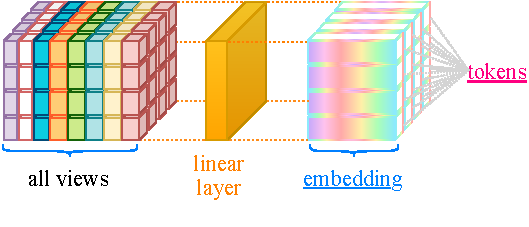
\includegraphics[height=0.18\linewidth]{img/cubes/SAT.pdf}} \vspace{-8pt} \\
        %     \multicolumn{3}{c}{\footnotesize $B \times \textcolor{myred}{\underline{W\!H}} \times \textcolor{myblue}{\underline{C_{SA}}}$} \\
        %     \multicolumn{3}{c}{\footnotesize (e) Spatial-angular Transformer.} \\
        % \end{tabular}
    \end{tabular}

    % \tabcolsep=0.20cm
    % \renewcommand{\arraystretch}{1}
    % \setlength{\medmuskip}{-1mu}
    % \begin{tabular}{ccccc}
    %     \includegraphics[width=0.1\linewidth]{img/cubes/LF.pdf} &
    %     \includegraphics[width=0.2\linewidth]{img/cubes/Spatial.pdf} &
    %     \includegraphics[width=0.2\linewidth]{img/cubes/Angular.pdf} &
    %     \includegraphics[width=0.2\linewidth]{img/cubes/EPI.pdf} &
    %     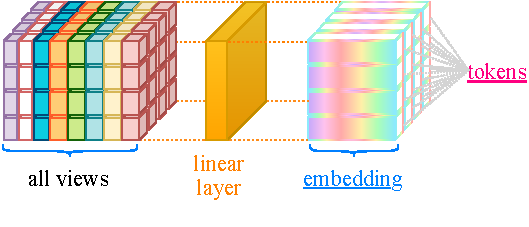
\includegraphics[width=0.2\linewidth]{img/cubes/SAT.pdf} \\
    %     \makecell{
    %         \footnotesize $U \times V \times W \times H \times C$ \\
    %         \footnotesize (a) LF image and tensor.
    %     } &
    %     \makecell{
    %         \footnotesize $U\!V \times \textcolor{myred}{\underline{W\!H}} \times \textcolor{myblue}{\underline{C}}$ \\
    %         \footnotesize (b) Spatial transformer. \\
    %     } &
    %     \makecell{
    %         \footnotesize $W\!H \times \textcolor{myred}{\underline{U\!V}} \times \textcolor{myblue}{\underline{C}}$ \\
    %         \footnotesize (c) Angular transformer. \\
    %     } &
    %     \makecell{
    %         \footnotesize $V\!H \times \textcolor{myred}{\underline{U\!W}} \times \textcolor{myblue}{\underline{C}}$ \\
    %         \footnotesize (d) EPI transformer. \\
    %     } &
    %     \makecell{
    %         \footnotesize $V\!H \times \textcolor{myred}{\underline{U\!W}} \times \textcolor{myblue}{\underline{C}}$ \\
    %         \footnotesize (e) Spatial-angular transformer. \\
    %     }
    % \end{tabular}
    \caption{Illustration of available data in LF tensors used by existing LF Transformers under the One-to-One scheme and our proposed Many-to-Many Transformer. For the tensors, each color represents a SAI.}
    \label{fig:Cubes}
\end{figure*}


\noindent{\bf Motivations.} The advances in deep learning, particularly convolutional neural networks (CNNs) \cite{yoon2017LFCNN, yeungSAS_LFSR2019, wangDistgSSR_TIP2022} and Vision Transformers (ViT) \cite{dosovitskiyViT_arXiv2020, liuSwin_ICCV2021, luESRT_CVPR2022}, have led to significant improvement in LFSR than traditional methods \cite{wanner2014variational}. The success has also extended to LFSR by processing 4D LF images in 2D subspaces, such as spatial, angular \cite{wangDPT_AAAI2022, liangLFT_SPL2022}, or Epipolar Image (EPI) \cite{liangEPIT_arXiv2023} subspaces. However, these methods predominantly suffer from subspace isolation, a defect causing sub-optimal performance.

Specifically, this issue arises when adapting 2D operations to the 4D LF data, existing approaches have to compromise its complete access to the LF information. This is primarily because training networks directly on voluminous 4D LF data, e.g. 4D convolutions \cite{yeungSAS_LFSR2019}, demands a relatively large number of weights, which is prone to optimization difficulties and heavy computation. As a workaround, most previous methods decompose the 4D data into 2D subspaces such as spatial and angular subspaces, or EPI subspaces. In implementation, one typical practice is to temporarily reshape a 4D tensor to expose two operative dimensions as tokens while merging the other two dimensions with the batch dimension. This decomposition enables 2D operations to perform on 4D LF tensors, and in training, the optimization is conducted on the whole tensor. However, a significant limitation arises during inference. When inferring the value at a specific location, access to the two merged dimensions is confined to only one location at a time, rather than spanning the entire dimensionality. As a result, even if with non-local Transformers, the effective receptive field is virtually restricted to a local context within the operative subspaces, leading to an One-to-One scheme.

For instance, consider the scenario depicted in Figure \ref{fig:Cubes}(a), where a single 4D LF tensor $I(u, v, x, y) \in \mathbb{R}^{U \times V \times W \times H \times C}$ is part of a batch $B$. Here, $(u, v, x, y)$ denotes a pixel's spatial location $(x, y)$ and angular location (or SAI) $(u, v)$. By merging the angular subspace $(U, V)$ into the batch dimension, a 2D spatial Transformer in Figure \ref{fig:Cubes}(b) is enabled to operate on the flatten spatial subspace $(W, H)$ as tokens across SAIs. However, this merging effectively isolates the network's forward propagation in the merged angular subspace $BUV$, as depicted by transparent blocks in the batch dimension. Consequently, the network is restricted to accessing only one SAI at a time during processing. This procedural constraint can be formally expressed as
\begin{equation} \label{eq:before}
\begin{split}
    I_{2}(u, v, x, y) = F \cdot \{I_{1}(\bar{u}, \bar{v}, \bar{x}, \bar{y})\}_{(\bar{u}, \bar{v}) = (u, v), (\bar{x}, \bar{y}) \in \mathbb{R}^{W \times H}}
    % I_{2}(u, v, x, y) = F({ \{I_{1}(u', v', x', y')\} }), & \quad (u', v') = (u, v) \\
    % & \quad (x', y') \in \mathbb{R}^{W \times H} \\
\end{split}
\end{equation}
where $F$ is a 2D operation, which can be either convolution or Transformers, and $I_{1}$ and $I_{2}$ are the input and output LF tensors of the operation. Under this scheme, to obtain a complete LF tensor, Equation \ref{eq:before} is repeated $U \times V$ times, each effectively being a One-to-One operation mapping from a SAI in $I_{1}$ at a single angular location $(u, v)$ to a SAI in $I_{2}$ at the same isolated angular location $(u, v)$ in the output. However, the ideal processing would instead use all SAIs to inform the computation loosening the constraint $(\bar{u}, \bar{v}) = (u, v)$, resulting in:
\begin{equation} \label{eq:after}
\begin{split}
    I_{2}(u, v, x, y) = F \cdot \{I_{1}(\bar{u}, \bar{v}, \bar{x}, \bar{y})\}_{(\bar{u}, \bar{v}, \bar{x}, \bar{y}) \in \mathbb{R}^{U \times V \times W \times H}}
\end{split}
\end{equation}

Subspace isolation is not unique to spatial Transformers and extends to other forms of data decomposition under the One-to-One scheme. For example, an angular Transformer is limited to accessing only one pixel across SAIs as depicted in Figure \ref{fig:Cubes}(c). Similarly, an EPI Transformer can only access a slice of two dimensions in the EPI subspace merged with the batch dimension, as shown in Figure \ref{fig:Cubes}(d). These constraints, inherent in the One-to-One operational scheme, significantly impede the ability of existing models to fully exploit the spatial and angular cues available in LF data, resulting in an incomplete spatial-angular representation.

\noindent{\bf Contributions.}
To address this issue, in this paper, we propose the novel Many-to-Many Transformer (M2MT), a new scheme to achieve the goal of comprehensive data integration outlined in Equation \ref{eq:after} and alleviate the isolation. The M2MT method begins by constructing correlation embeddings in the angular subspace. It then applies a self-attention mechanism to model long-range dependencies within the spatial subspace. This innovative approach allows the M2MT to access all the spatial and angular cues present in an LF image during each step of data propagation, thereby facilitating the creation of a holistic spatial-angular representation with a truly non-local context.

With M2MT as a foundational component, we present a simple yet effective network, M2MT-Net, incorporating M2MT in the spatial subspace and vanilla Transformers in the angular subspace. Through extensive experimental evaluation, we showcase M2MT-Net's outstanding performance, establishing it as a new state-of-the-art for LFSR.

Furthering the research, we delve into a series of analysis to discover the mechanisms behind its success. Particularly, by leveraging the technique of local attribution maps (LAM) \cite{guLAM_CVPR2021}, which visualize influential pixels, to gain interpretability of neural networks. Figure \ref{fig:First} reveals that M2MT utilizes more pixels across broader SAIs than the current state-of-the-art methods like EPIT \cite{liangEPIT_arXiv2023}. This observation substantiates the efficacy of M2MT, which mitigates the limitation of subspace isolation, simultaneously preserving more high-frequency cues in the spatial subspace and establishing a richer and non-local interplay of SAI dependencies in the angular subspace.

The contributions of this paper can be summarized as follows:
\begin{enumerate}
    \item The limitation of subspace isolation is identified, which predominantly impedes the performance of existing LF image processing methods by restricting data access when decomposing a 4D operation into a few One-to-One 2D operations.
    \item To overcome the limitations imposed by the One-to-One scheme, we introduce the Many-to-Many Transformer (M2MT), which aggregates correlation information from the angular subspace and performs a self-attention mechanism in the spatial subspace. A simple-yet-effective network, M2MT-Net, is developed incorporating the proposed M2MT for LFSR.
    \item Experimental results validate that M2MT-Net achieves state-of-the-art performance. In-depth analysis, especially the LAM analysis, is conducted to reveal its truly non-local context, utilizing all available information in a LF image for superior performance.
\end{enumerate}